\documentclass[10pt, compress]{beamer}

\usetheme{m}

\usepackage{booktabs}
\usepackage[scale=2]{ccicons}
\usepackage{minted}
\usepackage{tabularx}

\usepgfplotslibrary{dateplot}

\usemintedstyle{trac}

\title{Evaluación estratégica del uso de Gamification en ventas \emph{on-line}}
\subtitle{}
\date{27 de Abril, 2015}
\author{Ignacio j. Villacura de la Paz}
\institute{Departamento de Informática\\ Universidad Técnica Federico Santa María}

\begin{document}

\maketitle

\section{Introducción}

\begin{frame}[fragile]
  \frametitle{Contenidos}

\begin{columns}[onlytextwidth]
 \column{0.5\textwidth}
  \begin{itemize}[<+- | alert@+>]
    \item Motivación.
    \item \emph{Gamification}
	\begin{itemize}[<+- | alert@+>]
	  \item Definición.
	  \item Usos cotidianos.
	\end{itemize}
    \item Problemática:
	\begin{itemize}[<+- | alert@+>]
          \item Definición.
          \item Tienda ayudante.
        \end{itemize}
    \item Solución propuesta:
	\begin{itemize}[<+- | alert@+>]
          \item Descripción.
          \item Sistema Base.
	  \item Herramientas utilizadas.
	  \item Encuesta evaluativa.
        \end{itemize}
\end{itemize}

 \column{0.5\textwidth}
  \begin{itemize}[<+- | alert@+>]
    \item Datos Experimentales:
	\begin{itemize}[<+- | alert@+>]
          \item Resultados implementación.
          \item Resultados encuesta.
        \end{itemize}
    \item Conclusiones.
    \item Trabajos futuros.
  \end{itemize}
\end{columns}
\end{frame}

\begin{frame}[fragile]
  \frametitle{Motivación}
\begin{columns}[onlytextwidth]
 \column{0.5\textwidth}
\begin{itemize}
\item Entrada de multinacionales \\
al mercado nacional.
\item PyMe. 
\item E-commerce y autogestión.
\end{itemize}

 \column{0.5\textwidth}
\begin{figure}
\centering
    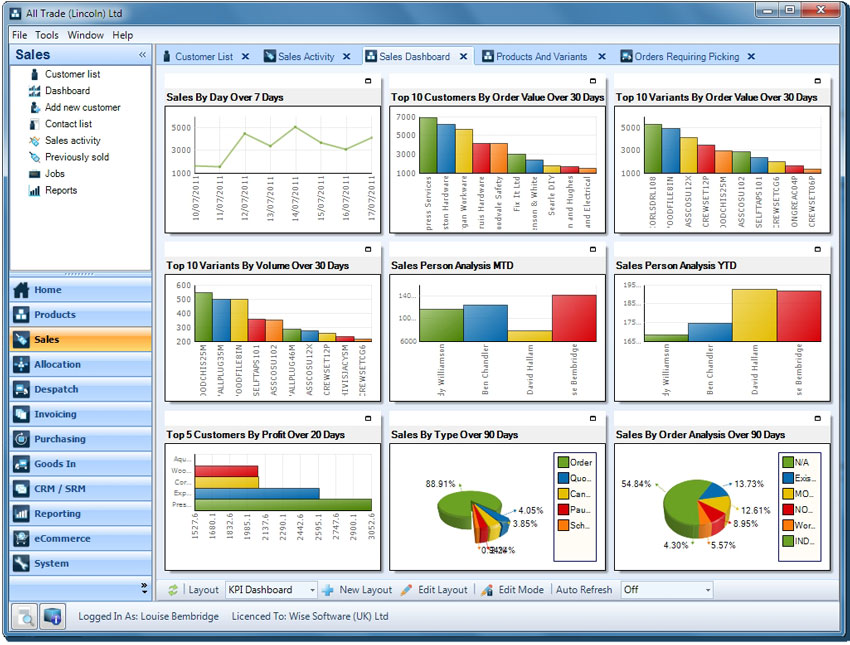
\includegraphics[width=0.8\textwidth]{images/SalesDashboard.jpg}
    \caption{Dashboard sistema de ventas.}
    \label{fig:awesome_image}
\end{figure}
\end{columns}
\end{frame}

\section{\emph{Gamification}}

\begin{frame}[fragile]
  \frametitle{Definición}
  \begin{description}
    \item[\textbf{\emph{Gamification}}] ``Es el uso de elementos del diseño de juego en contextos diferentes al de 
juego''.
  \end{description}

\end{frame}

\begin{frame}
\frametitle{Definición}

\begin{description}
 \item[\textbf{Juego}] En primer lugar este concepto se refiere al juego en su totalidad, y no a la acción de jugar. 
Este concepto es caracterizado por un conjunto de reglas explicitasıcitas, que crean un ambiente en donde los 
jugadores buscan la competición para completar objetivos y metas.
 \item[\textbf{Elementos del diseño de juego}] Los elementos a utilizar son característicos a los juegos, que se 
encuentran en la mayoría de ellos y que cumplen un rol importante en su jugabilidad.
 \item[\textbf{Contextos diferentes al de juego}] Existe fuera de un juego o de un ambiente que contiene gamification.
\end{description}
\end{frame}

\begin{frame}
 \frametitle{Usos cotidianos}
\begin{columns}[onlytextwidth]
\column{0.5\textwidth}

        \begin{itemize}[<+- | alert@+>]
          \item Puntos \emph{retail}.
          \item Canje de productos.
	  \item Obtención de logros.
        \end{itemize}

\column{0.5\textwidth}
\begin{figure}
\centering
    
\includegraphics[width=0.8\textwidth]{images/retail.png}
    \caption{Puntos mas utilizados.}
    \label{fig:awesome_image}
\end{figure}
\end{columns}
\end{frame}

\section{Problemática}
\begin{frame}
\frametitle{Definición}
        \begin{itemize}[<+- | alert@+>]
          \item Diferencias entre PyMes y grandes empresas, en ventas \emph{on-line}, debido a la diferencia de recursos.
	  \item PyMe y empleos.
	  \item Acceso de PyMe a tecnologías actuales para venta \emph{on-line}.
        \end{itemize}

\begin{table}[h]
\footnotesize
\centering
\begin{tabular}{|l|c|c|c|}
\hline
{\bf Empresa}  & {\bf Número de Trabajadores} & {\bf Porcentaje de ocupación} & {\bf Ventas anuales}\\
\hline
Micro    & 1 a 4                & 44.4\%  & menos de 2400 UF\\
\hline
Pequeña  & 5 a 49               & 37\%  & 2401 a 25000 UF\\
\hline
Mediana  & 50 a 199             & 13\%  & 25001 a 100000 UF\\
\hline
Grande   & más de 199           & 10\%  & más de 100000 UF\\
\hline
\end{tabular}
\caption{Tamaño de empresa según cantidad de empleados.}
\label{tab:tam_empresa}
\end{table}
\end{frame}

\begin{frame}
 \frametitle{Tienda}

Se contó con la ayuda de la tienda ``Kurgan''. Esta cedió el espacio para implementar el sistema de ventas 
propuesto como solución.

\begin{columns}[onlytextwidth]
\column{0.5\textwidth}
\begin{figure}
\centering
    
\includegraphics[width=0.8\textwidth]{images/logo.png}
    \caption{Logo tienda ``Kurgan''.}
    \label{fig:awesome_image}
\end{figure}

\column{0.5\textwidth}
\begin{figure}
\centering
    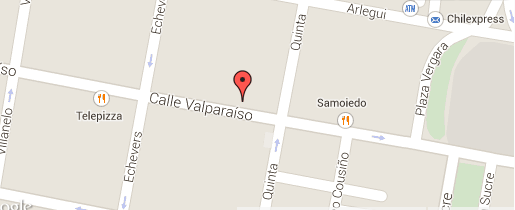
\includegraphics[width=0.8\textwidth]{images/mapa.png}
    \caption{Ubicación tienda ``Kurgan''}
    \label{fig:awesome_image}
\end{figure}

\end{columns}
\end{frame}

\section{Solución Propuesta}

\begin{frame}
 \frametitle{Descripción}

\begin{itemize}[<+- | alert@+>]
 \item Sistema de ventas \emph{on-line}.
 \item Fácil administración.
 \item Utilización de \emph{gamification} para atraer y retener clientes.
\end{itemize}
\end{frame}

\begin{frame}
 \frametitle{Características Solución}
\begin{description}
 \item[\textbf{Bajo costo}] Debido a los escasos recursos que poseen las PyMes es necesario e importante que
la solución tenga requiera los mínimos recursos posibles.
 \item[\textbf{Facilidad de configuración}] El sistema debe poder ser configurado por el usuario.
 \item[\textbf{Facilidad de administración}] El sistema debe poder ser administrado por el usuario.
\end{description}
\end{frame}

\begin{frame}
 \frametitle{Características Sistema Base}

\begin{itemize}[<+- | alert@+>]
 \item Facilidad de instalación.
 \item Facilidad de administración.
 \item Actualizaciones y comunidad activa.
 \item Características utilizables.
 \item Traducciones.
\end{itemize}
\end{frame}

\begin{frame}
 \frametitle{Sistema Base}

\begin{figure}
\centering
    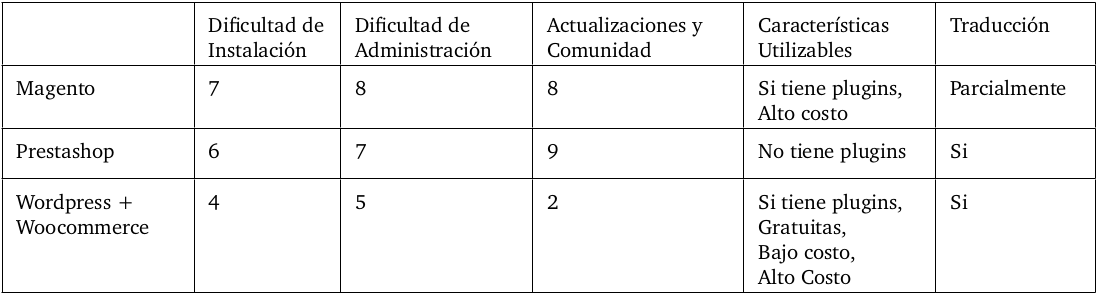
\includegraphics[width=0.9\textwidth]{images/tablaWord.png}
    \caption{Tabla comparativa de sistemas bases.}
    \label{fig:awesome_image}
\end{figure}

\end{frame}

\begin{frame}
 \frametitle{Herramientas Utilizadas}

\begin{itemize}[<+- | alert@+>]
 \item Woocommerce: Herramienta que modifica el sistema base en tienda on-line.
 \item WooCube Pro: Plugin dedicado a la entrega y guardado de los puntos.
 \item WPAchievement: Da la funcionalidad de entregar logros al realizar completamente una tarea.
 \item Refer a Friend: Herramienta que ayuda al usuario a invitar a amigos y obtener beneficios con ésto.
\end{itemize}
\end{frame}

\begin{frame}
 \frametitle{Encuesta Evaluativa}

Encuesta con los objetivos:

\begin{itemize}[<+- | alert@+>]
 \item Apoyo de la investigación.
 \item Conocimiento de la población sobre \emph{gamification}.
 \item Interacción de la población con \emph{gamification}.
\end{itemize}
\end{frame}

\section{Resultados}

\begin{frame}
 \frametitle{Resultados Implementación}

En primera instancia, se debió establecer los beneficios a entregar:

\begin{itemize}
\item \textbf{Registro en la tienda:} 500 puntos.
\item \textbf{Puntos por venta:} 10\% del total de la compra.
\item \textbf{Comentarios:} 100 puntos.
\item \textbf{\emph{Referals}:} Cupón de 5\% en total venta.
\end{itemize}
\end{frame}

\begin{frame}
 \frametitle{Resultados Implementación - Pre-\emph{Gamification}}

Antes de implementar \emph{gamification} se obtuvieron datos por $30$ días para poder
compararlos una vez el sistema completo fuera implementado.

\begin{itemize}
    \item \textbf{Cantidad de visitas:} 315 (visitas únicas).
    \item \textbf{Cantidad de lecturas:} 445.
    \item \textbf{Cantidad de usuarios inscritos:} 0.
    \item \textbf{Cantidad de ventas realizadas:} 0.
\end{itemize}

\end{frame}

\begin{frame}
 \frametitle{Resultados Implementación - Post-\emph{Gamification}}

Una vez terminada la etapa de recolección de datos, se implemento \emph{gamification}. Esta
etapa tuvo una duración de $30$ días y se obtuvieron los siguientes datos:

\begin{itemize}
    \item \textbf{Cantidad de visitas:} 476 (visitas únicas).
    \item \textbf{Cantidad de lecturas:} 641.
    \item \textbf{Cantidad de usuarios inscritos:} 0.
    \item \textbf{Cantidad de ventas realizadas:} 0.
\end{itemize}

\end{frame}


\begin{frame}
 \frametitle{Resultados Implementación - Análisis de datos}

Al analizar los datos se puede concluir lo siguiente:

\begin{itemize}[<+- | alert@+>]
 \item Aumento en la cantidad de visitas.
 \item No hubo aumento de usuarios registrados.
 \item Implementación de \emph{gamification} no fue efectiva.
\end{itemize}

\begin{table}[h]
\footnotesize
\centering
\resizebox{\linewidth}{!}{
\begin{tabular}{|l|c|c|c|c|}
\hline
  & {\bf Cantidad de visitas} & {\bf Cantidad de lecturas} & {\bf Cantidad de usuarios inscritos} & {\bf Cantidad de ventas realizadas}\\
\hline
Pre Implementación    & 315  & 445  & 0 & 0\\
\hline
Post Implementación  & 476 & 641  & 0 & 0\\
\hline
\end{tabular}}
\caption{Datos Pre y Post implementación.}
\label{tab:tam_empresa}
\end{table}

\end{frame}

\begin{frame}
 \frametitle{Resultados Encuesta}

Debido a que los datos no fueron concluyentes para decir si \emph{gamification} es una herramienta útil. 
Se realizo una encuesta para complementar la información obtenida:

\begin{itemize}
    \item \textbf{Intervalo de confianza:} 95\%.
    \item \textbf{Error Muestral:} 7.5\%.
    \item \textbf{Cantidad mínima de respuestas:} 165\%.
    \item \textbf{Universo poblacional:} 180 personas.
    \item \textbf{Numero de Preguntas:} 12.
    \item \textbf{Sexo:} 71\% Masculino y 29\% Femenino.
\end{itemize}

\end{frame}

\begin{frame}
 \frametitle{Resultados Encuesta}

\begin{table}[h]
\centering
\footnotesize
\begin{tabular}{| p{6cm} | c | c | c |}
\hline
                          {\bf Pregunta}
                        & {\bf Si(\%)}
                        & {\bf No(\%)}
                        & {\bf Total} \\ \hline
¿Está al tanto de lo que es \emph{gamification}?&57\%&43\%&180 \\ \hline
¿Usted acumula puntos de grandes empresas?&56\%&44\%&180 \\ \hline
¿Está al tanto de los beneficios que dicha empresa le ofrece?&75\%&25\%&92 \\ \hline
¿Ha utilizado éstos beneficios en algún momento?&79\%&21\%&100 \\ \hline
¿Cree usted que el uso de \emph{gamification} lo motiva a volver a la tienda?&68\%&32\%&180 \\ \hline
\end{tabular}
\caption{Tabla de respuestas para preguntas de respuesta Si o No}
\end{table}
\end{frame}

\begin{frame}
 \frametitle{Resultados Encuesta}

\begin{table}[h]
\centering
\footnotesize
\resizebox{\linewidth}{!}{
\begin{tabular}{|p{5cm}|c|c|c|}
\hline
{\bf Pregunta} & {\bf Presencial (persona a persona)(\%)} & {\bf On-line (vía internet)(\%)} & {\bf Total}\\
\hline
¿Cuál es su preferencia a la hora de realizar compras?& 26\% & 74\% & 180 \\
\hline
\end{tabular}}
\caption{Tabla de respuesta para pregunta de la encuesta: {\bf ¿Cuál es su preferencia a la hora de realizar compras?}}
\label{tab:Preg8}
\end{table}


\end{frame}

\begin{frame}
 \frametitle{Resultados Encuesta}

\begin{table}[h]
\centering
\footnotesize
\resizebox{\linewidth}{!}{
\begin{tabular}{|p{4cm}|c|c|c|}
\hline
{\bf Pregunta} & {\bf Tienda on-line con \emph{gamification}(\%)} & {\bf Tienda on-line convencional(\%)} & {\bf Total}\\
\hline
¿Prefiere un sitio de ventas on-line con \emph{gamification} o un sitio convencional?& 69\% & 31\% & 180 \\
\hline
\end{tabular}}
\caption{Tabla de respuesta para pregunta de la encuesta: {\bf ¿Prefiere un sitio de ventas on-line con
\emph{gamification} o un sitio convencional?}}
\label{tab:Preg9}
\end{table}


\end{frame}

\begin{frame}
 \frametitle{Resultados Encuesta}

\begin{table}[h]
\centering
\footnotesize
\begin{tabular}{|l|c|c|c|c|c|c|}
\hline
 & \multicolumn{6}{c|}{{\bf Preferencias(\%)}} \\
\hline
{\bf Opciones} & {\bf 1} & {\bf 2} & {\bf 3} & {\bf 4} & {\bf 5} & {\bf Total}\\
\hline
Precios Bajos & 1\% & 1\% & 5\% & 13\% & 80\% & 180\\
\hline
Acumulación de puntos & 23\% & 22\% & 21\% & 17\% & 17\% & 180\\
\hline
Descuentos en compras & 7\% & 14\% & 18\% & 29\% & 32\% & 180\\
\hline
Obtención de productos exclusivos & 24\% & 17\% & 25\% & 16\% & 18\% & 180\\
\hline
Reconocimiento publico & 82\% & 7\% & 6\% & 2\% & 3\% & 180\\
\hline
\end{tabular}
\caption{Tabla de respuestas para pregunta de la encuesta: {\bf ¿Qué beneficios prefiere o preferiría obtener?}}
\label{tab:Preg7}
\end{table}

\end{frame}

\section{Conclusiones}

\begin{frame}
 \frametitle{Conclusiones}

\begin{itemize}
\item \emph{Gamification} es una herramienta útil para mejorar ventas.
\item Las herramientas utilizadas son suficientes para una PyMe.
\item El usuario del sistema web debe creer en él. Con esto poder entregar beneficios que al cliente 
le sean atractivos 
\item La población ya conoce el concepto y le atrae que las empresas lo utilicen.
\end{itemize}
\end{frame}

\begin{frame}
 \frametitle{Trabajos futuros}

\begin{itemize}

\item Realizar un análisis de estrategias de marketing que ayuden, en un inicio, a promocionar la nueva 
implementación de \emph{gamification} en una tienda virtual.
\item Implementación de los otros sistemas bases con el objetivo de realizar una comparación mas exhaustiva
de estas herramientas.
\item Investigar y utilizar otra forma de entrega de beneficios.
\end{itemize}
\end{frame}

\plain{¿Preguntas?}

\end{document}
